\begin{figure*}[t]
    \centering
    
    \begin{tabular}{c c c c}
    	
    	{(1)} &
    	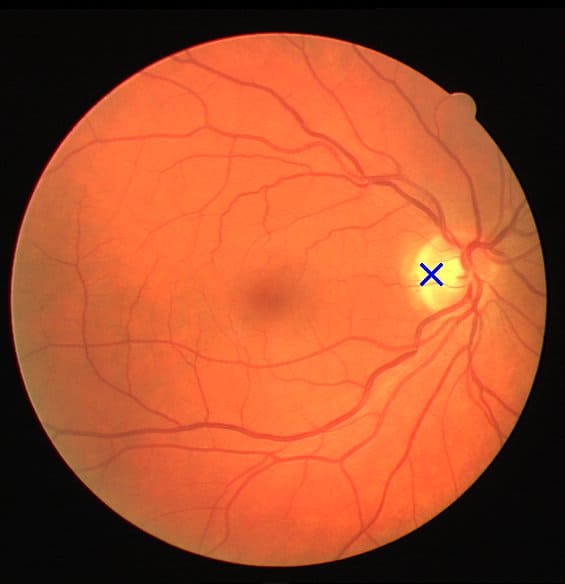
\includegraphics[width=3.0cm]{Images/Methode/Detection/Drive/02_test.jpg}{(a)} & 
    	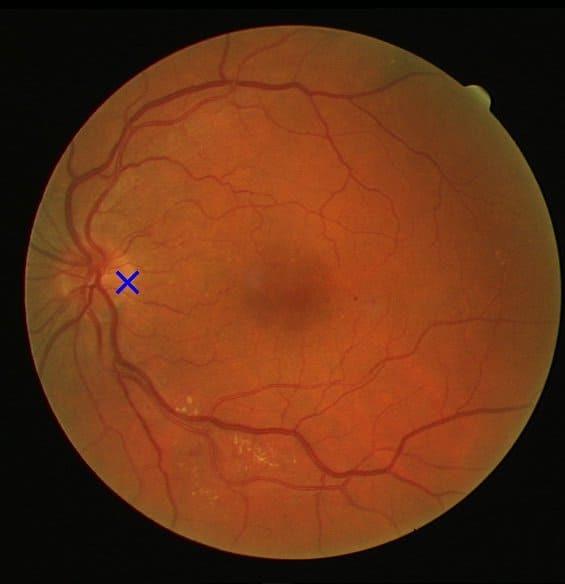
\includegraphics[width=3.0cm]{Images/Methode/Detection/Drive/03_test.jpg}{(b)} &
    	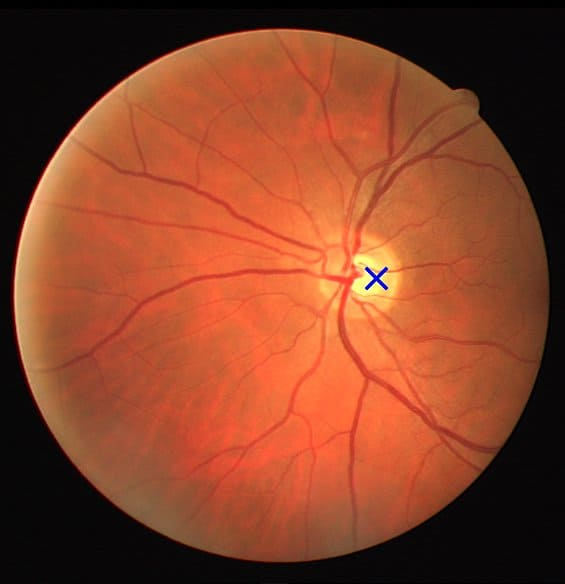
\includegraphics[width=3.0cm]{Images/Methode/Detection/Drive/04_test.jpg}{(c)} \\
    	
    	{} &
    	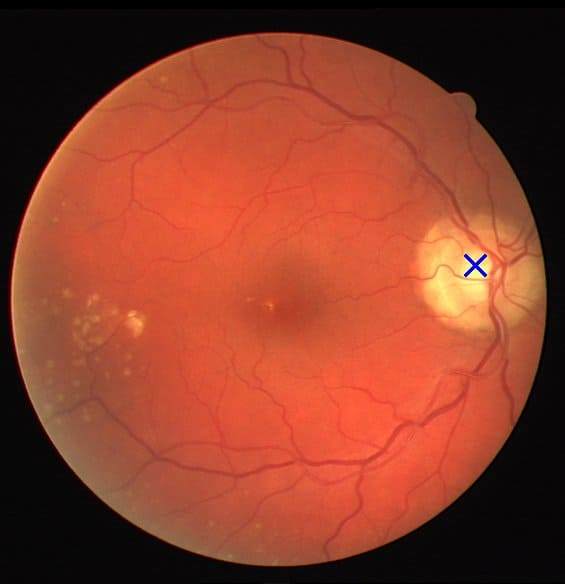
\includegraphics[width=3.0cm]{Images/Methode/Detection/Drive/08_test.jpg}{(d)} & 
    	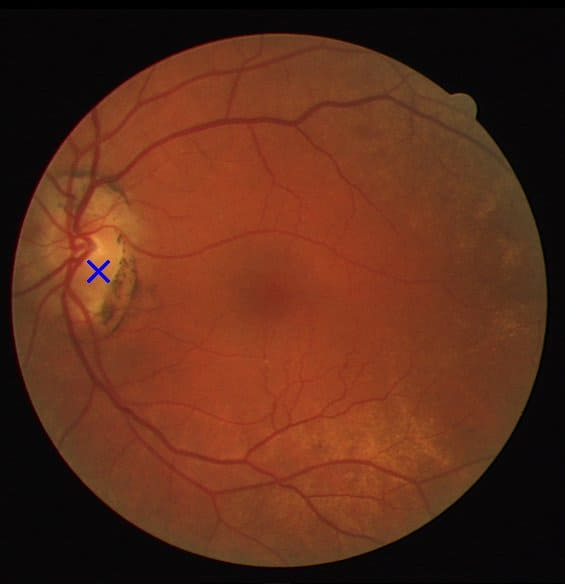
\includegraphics[width=3.0cm]{Images/Methode/Detection/Drive/26_training.jpg}{(e)} &
    	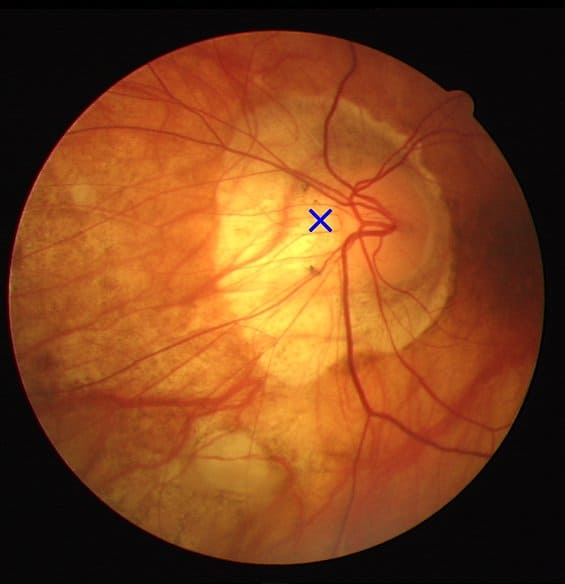
\includegraphics[width=3.0cm]{Images/Methode/Detection/Drive/34_training.jpg}{(f)} \\
    	
    	{(2)} &
    	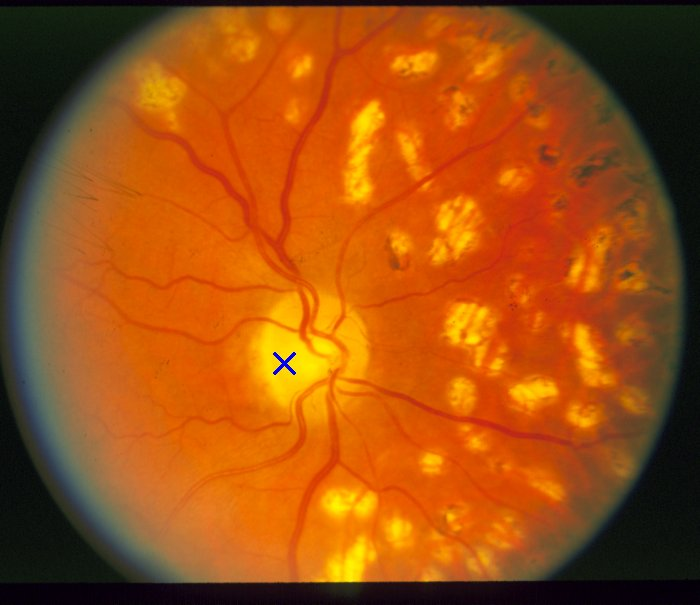
\includegraphics[width=3.0cm]{Images/Methode/Detection/Stare/im0179.jpg}{(g)} & 
    	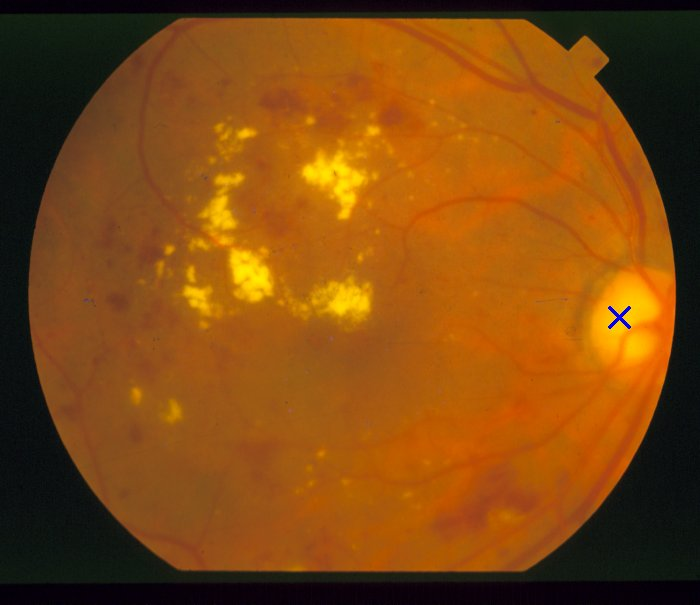
\includegraphics[width=3.0cm]{Images/Methode/Detection/Stare/im0096.jpg}{(h)} &
    	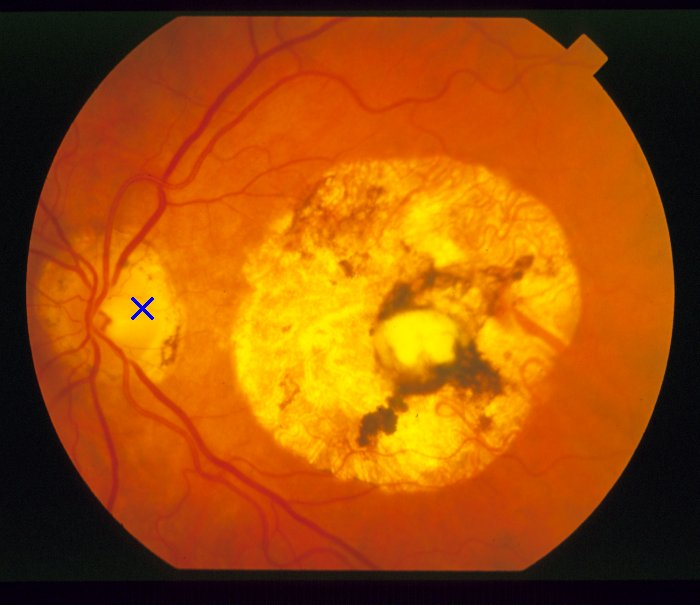
\includegraphics[width=3.0cm]{Images/Methode/Detection/Stare/im0110.jpg}{(i)} \\
    	
    	{} &
    	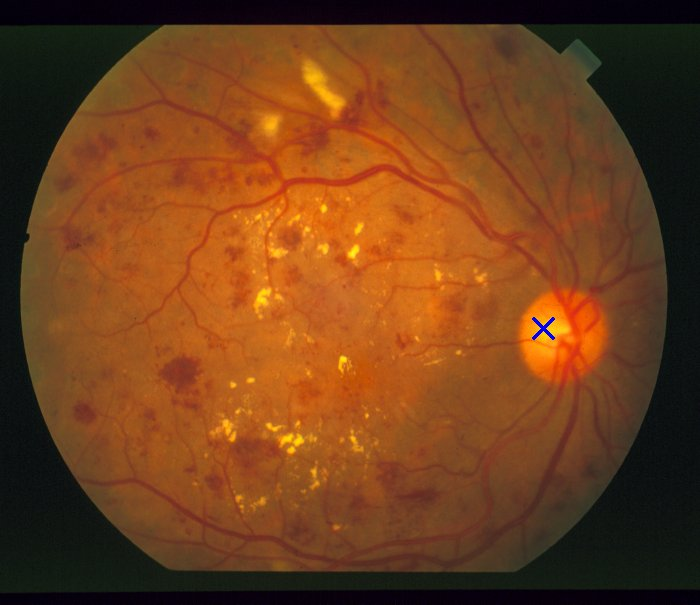
\includegraphics[width=3.0cm]{Images/Methode/Detection/Stare/im0140.jpg}{(j)} & 
    	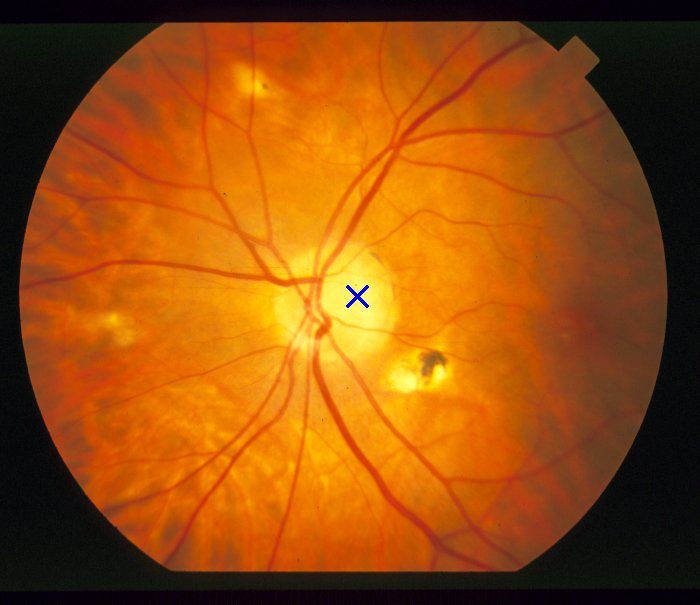
\includegraphics[width=3.0cm]{Images/Methode/Detection/Stare/im0183.jpg}{(k)} &
    	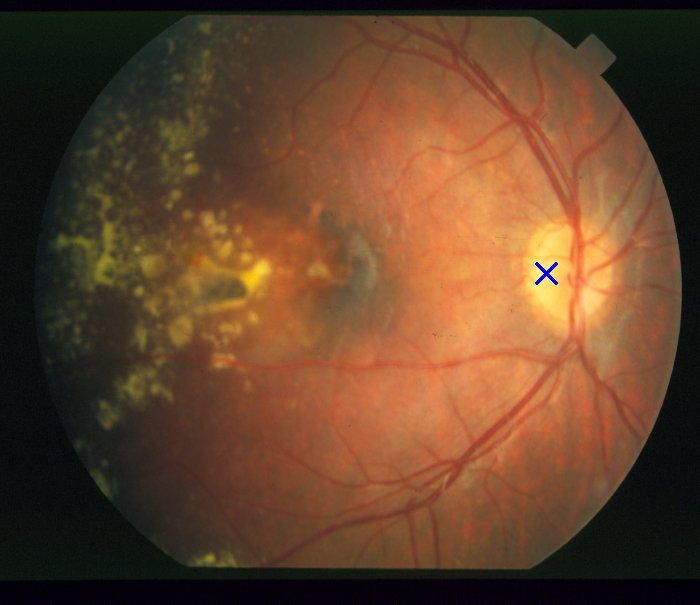
\includegraphics[width=3.0cm]{Images/Methode/Detection/Stare/im0177.jpg}{(l)} \\
    \end{tabular}

    
    \caption{\label{examples_detection}OD detection examples, in both healthy (1) and non-healthy (2) databases. The blue cross ($\times$) represents the found OD location point ((1) DRIVE database (six samples a, b, c, d, e, f), (2) STARE database (six samples g, h, i, j, k, l)).}
\end{figure*}
